\documentclass[aps,twocolumn,secnumarabic,balancelastpage,amsmath,amssymb,nofootinbib,floatfix]{revtex4-1}

\usepackage{graphicx}      % tools for importing graphics
\usepackage[colorlinks=true]{hyperref}  % this package should be added 
\usepackage{dcolumn}% Align table columns on decimal point
\usepackage{bm}% bold math
\usepackage{xcolor}

\newcommand{\ev}{\,{\rm eV}}
\newcommand{\nm}{\,{\rm nm}}
\newcommand{\pA}{\,{\rm pA}}
\newcommand{\V}{\,{\rm V}}
\newcommand{\Js}{\,{\rm J}\,{\rm s}}


\begin{document}

\title{Photoelectric Effect}

\author{Vinh Tran}
\affiliation{Department of Physics and Kavli Institute for Astrophysics and Space Research, Massachusetts Institute of Technology, Cambridge, MA 02139, USA}
\email{vinhtran@mit.edu}

\date{\today}

%%%%%%%%%%%%%%%%%%%%%%%%%%%%%%%%%%%%%%%%%%%%%%%%%%%%%%%%%%%%%%%%%%

\begin{abstract}

We present a measurement of the Plank constant $h$ and the work function of the material $\phi$ from the cutoff voltages $V_{\rm{cut\,off}}$ at different wavelengths. The values of $V_{\rm{cut\,off}}$ are determined by bi-segment fits to the photoelectric currents $I_{\rm{pe}}$ as functions of the retarded voltages $V$ for the wavelengths of $\lambda = 365.0, \, 404.7, \, 435.8,$ and $546.1\nm$. The Plank constant $h$ and the work function $\phi$ are then fitted, with the results of $h = 6.30 \pm 0.63^{\rm{stat}} \pm 0.32^{\rm{sys}} \times 10^{-34}\Js$ and $\phi = 1.81 \pm 0.29^{\rm{stat}} \pm 0.18^{\rm{sys}}\ev$. The large statistical uncertainties in $h$ and $\phi$ are due to the correlation between the fitted values of the two parameters and can be reduced with a more diverse range of wavelengths. The systematic errors are mainly due to the uncertainties in the cutoff voltage measurements and can be reduced with a more precise apparatus. The value of $h$ is relatively consistent with the literature value of $h = 6.63 \times 10^{-34}\Js$. Future work may include the use of a more precise apparatus and a wider range of wavelengths to reduce the uncertainties in the measurements.

\end{abstract}

\maketitle

%%%%%%%%%%%%%%%%%%%%%%%%%%%%%%%%%%%%%%%%%%%%%%%%%%%%%%%%%%%%%%%%%%

\section{Introduction}
\label{sec:intro}

The photoelectric effect, first discovered by Heinrich Hertz~\citep{1Hertz887} in 1887 and later explained by Albert Einstein~\cite{Einstein1905} in 1905, describes the process in which charge particles are released from the metal surface by light of short-enough wavelength $\lambda$. In his work, Einstein characterized light as quanta of energy $h \nu$, with $h$ as the Plank constant and $\nu = c/\lambda$ as the light wave frequency. These light particles (i.e. photons) deposit energy into the charge particles (typically electrons) and push them out of the metal surface, overcoming the potential well. The depth of these potential wells, called the work function $\phi$, can be calculated as the difference between the photon energy $h \nu$ and the ejected charge particle's kinetic energy $K$
\begin{equation}
    \label{eqn:work_function}
    h \nu = K + \phi.
\end{equation}
A more general summary of the photoelectric effect can be found in the review by Klassen~\citep{Klassen2011}.

In this experiment, we perform a measurement of the Plank constant $h$ through the identification of the work function $\phi$ and the cutoff voltages, i.e. the voltages at which the photoelectric current is zero, for different wavelengths. In Section~\ref{sec:experiment}, we describe the experimental apparatus and the data collection process. In Section~\ref{sec:result}, we present the results of the experiment and discuss the implications of the measurements. Finally, in Section~\ref{sec:conclusion}, we summarize the findings and provide a conclusion.


\section{Experiment Setup}
\label{sec:experiment}

\subsection{Apparatus}
\label{sec:apparatus}

\begin{figure}
    \centering
    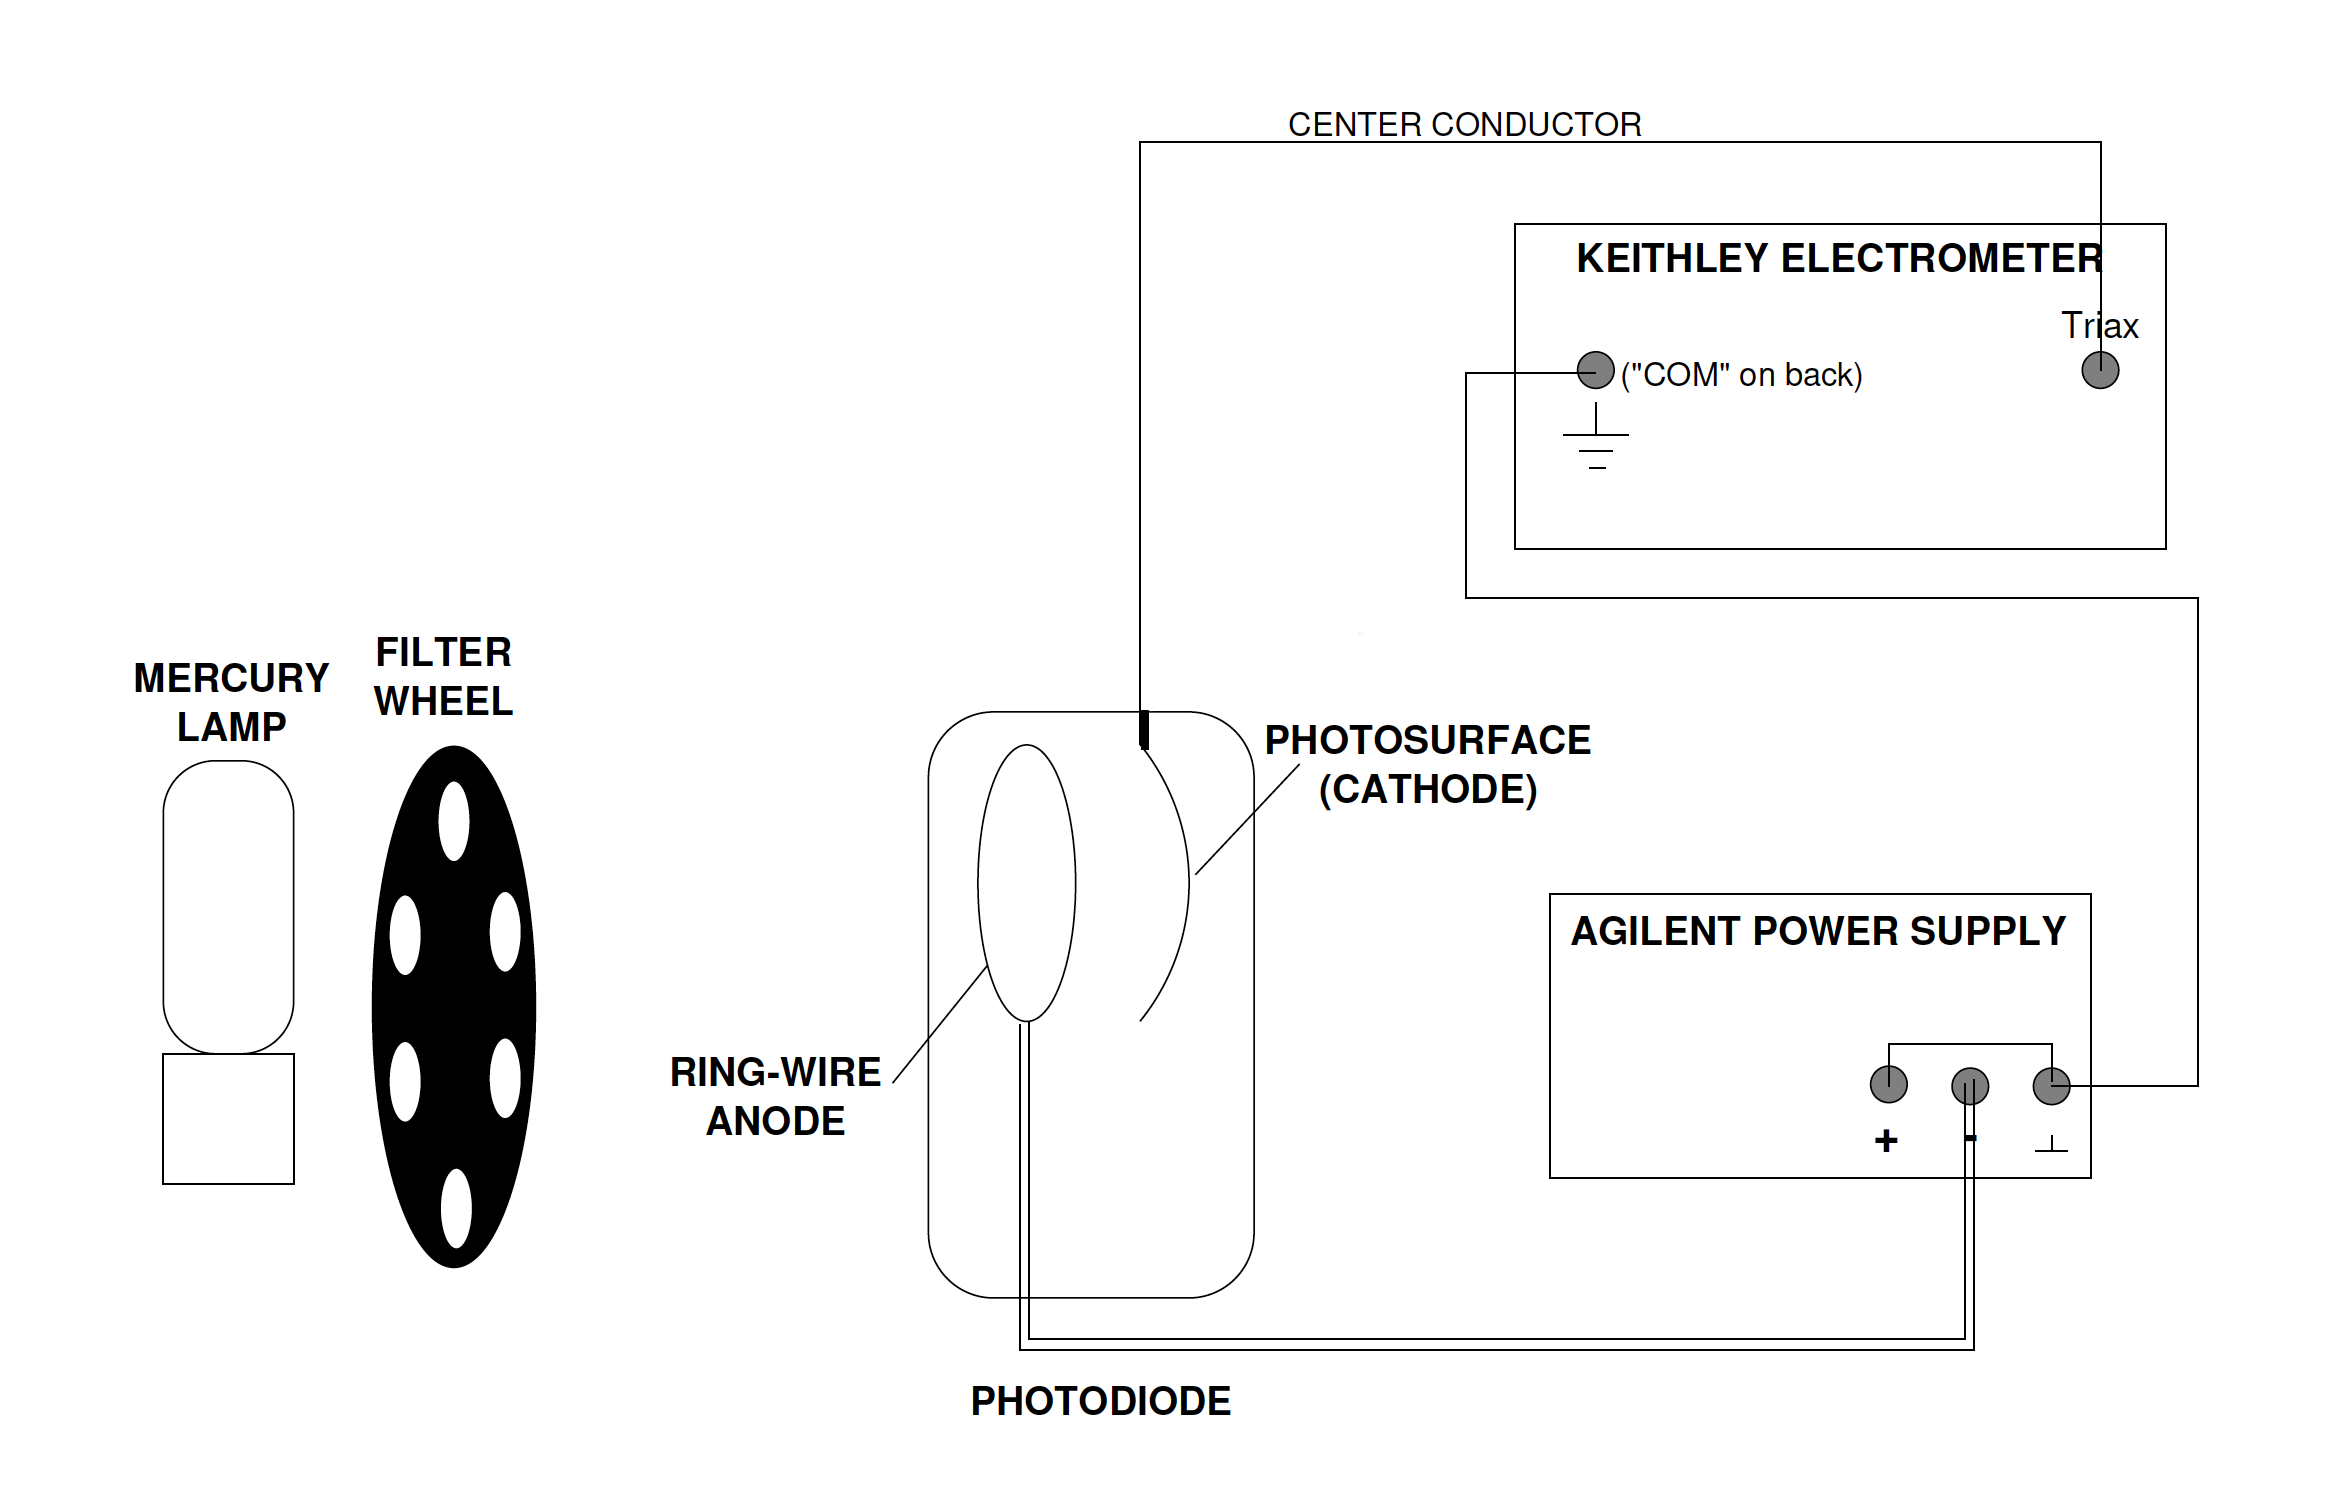
\includegraphics[width=0.49 \textwidth]{Figures/apparatus.png}
    \caption{The experiment apparatus, reconstructed from~\citep{MITPhotoelectricEffect}.}
    \label{fig:apparatus}
\end{figure}

The experiment utilizes the photoelectric apparatus shown in Figure~\ref{fig:apparatus}, following~\citep{MITPhotoelectricEffect}, which consists of a mercury lamp, a filter wheel, a photodiode, which comprises of a potassium photosuface (cathode) and a platinum-rhodium alloy ring wire (anode) with significantly higher work function compared to the photosurface, a voltage supply, and a Keithley electrometer. We pay special attention to the grounding of equipment and the alignment of apparatus to ensure the accuracy of the measurements. The positive terminal of the power supply is connected to the ground terminal and to the cathode of the photodiode (with the Keithley electrometer connected in between), while the power supply's negative terminal is connected to the photodiode's anode. This create a reverse (retarded) voltage $V$ across the photodiode, which can be adjusted to control the photoelectric current. The mercury lamp emits sharp emission peaks at different wavelengths, which can be selected by the filter wheel. We perform measurements for the wavelengths of $\lambda = 365.0, \, 404.7, \, 435.8,$ and $546.1\nm$, with the bandwidth of the filters of the order of $4.0\nm$. Light is then directed to the photosurface of the photodiode's cathode, where a current $I$ is generated for photons of sufficient energy, i.e. enough to overcome the work function $\phi$ and the retarded voltage $V$. The current is then measured by the Keithley electrometer. We look for the cutoff voltage $V_{\rm{cut\,off}}$, at which the energy of photon is barely sufficient for a non-zero current. Idealistically, this would be a sharp cutoff in terms of the photoelectric current, but in practice, the current gradually reduces as the voltage increases, as discussed in the following Subsection.

\subsection{Data Collection}
\label{sec:data_collection}

As demonstrated by various experiments~\citep[e.g.][]{Millikan1916,Quinn1964,Wong2011}, the voltage boundary manifests not as a clear cut off, but rather as a gradual reduction in currect, approaching an asymptotic flat regime. Additionally, as the retarded voltage further increase, the phenomenon of reverse current, where photoelectons emitted from light hitting the anode travel toward the cathode, occurs. Adapting our data collection stratergy according to these phenomenon, we measure the photoelectric current across a wide range of retarded voltages using semi-uniform steps. 

The current $I$ is typically of the order of $10 \text{--} 100\pA$, so further precautions in the apparatus arangement, e.g. the arangement and length of connecting wires, are required. At these scales, the fluctuation of the current also appears to be of important. Therefore, at each voltage, we record the different values of $I$ and obtain the central value $\mu_I$ and standard deviation $\sigma_I$ following the Bayesian principle with equal probability priors $p(\boldsymbol{\theta})$, where $\boldsymbol{\theta} = (\mu_I,\sigma_I)$, and the maximum a piori cost $C_{\rm{MAP}} (\boldsymbol{\theta} - \boldsymbol{\theta^\prime}) = \delta (\boldsymbol{\theta} - \boldsymbol{\theta^\prime})$. The values of $\mu_I$ and $\sigma_I$ follow
\begin{equation}
    \label{eqn:I_bayesian}
    \mu_I,\sigma_I =  \arg \min_{\mu_I,\sigma_I} - 2 \log{\mathcal{L} (\mu_I,\sigma_I)},
\end{equation}
where
\begin{equation}
    \label{eqn:I_NLL}
    - 2 \log{\mathcal{L} (\mu_I,\sigma_I)} = N \log{2 \pi \sigma_I^2} + \sum_i \left(\frac{I_i - \mu_I}{\sigma_I}\right)^2
\end{equation}
is the negative log likelihood function, $N$ is the number of measurements, and $I_i$ is the current at the $i$-th measurement. Onward, we denote $\mu_I$ as $I$ for simplicity. The approach performs well as the residual sum of squares (RSS) $\chi^2 = \sum_i (I_i - I)^2 / \sigma_I^2$ exhibit the typical expected value of the $\chi^2$ distribution of $N$ degrees of freedom.

To isolate the photoelectric effect from the background signal and other voltage-dependent effects, we also measure the currents at the same voltages but with the light source blocked. The background current $I_{\rm{bg}}$ is then subtracted from the total current $I_{\rm{total}}$ to obtain the photoelectric current $I_{\rm{pe}} = I_{\rm{total}} - I_{\rm{bg}}$.


\section{Results}
\label{sec:result}

\begin{figure}
    \centering
    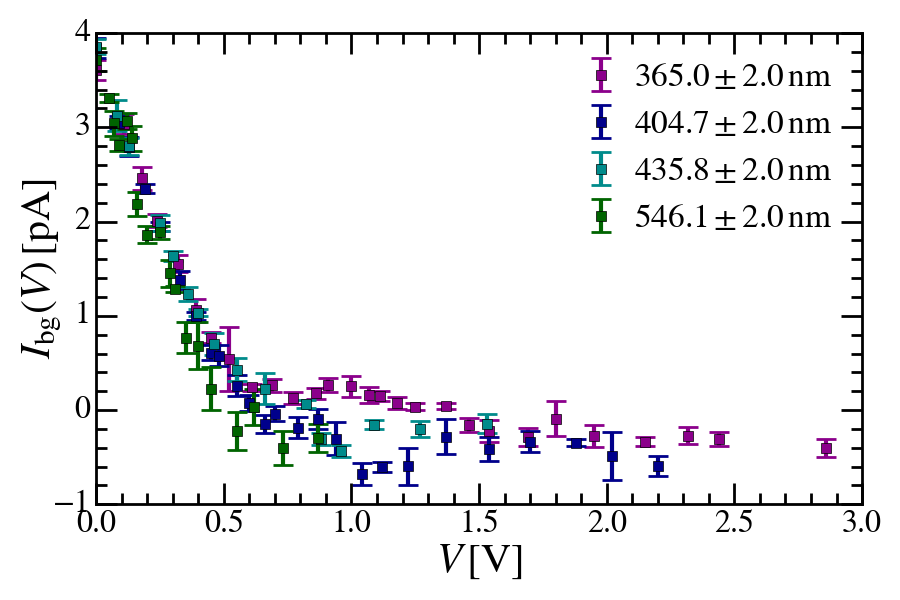
\includegraphics[width=0.49 \textwidth]{Figures/background.png}
    \caption{The background currents $I_{\rm{bg}}$ as functions of the retarded voltage $V$ for different wavelengths. The background currents remain consistent between different measurements, exhibiting a downward trend at the smaller $V$ regime. In general, the background currents are relatively small compared to the photoelectric current, but they are still significant enough to be subtracted from the total current, especially at the regions surrounding the cutoff voltage.}
    \label{fig:background}
\end{figure}

Fig.~\ref{fig:background} shows the voltage-dependency of the background currents at different wavelengths. We observe that across wavelengths, the backgrounds remain consistent, which is as expected with the light source blocked. Below $V = 1\V$, the background currents exhibit a downward trend, which may be due to some unknown voltage-dependent effects in the photodiode. Above $V = 1\V$, the background currents remain relatively constant, fluctuating around $-0.2 \text{--} 0.4\pA$. The background currents are relatively small compared to the photoelectric currents. However, they are still significant enough to affect the measurements at the regions surrounding the cutoff voltage, especially with $V_{\rm{cut\,off}} \lesssim 1\V$.

\subsection{Cut Off Voltages}
\label{sec:cut_off_voltages}

\begin{figure}
    \centering
    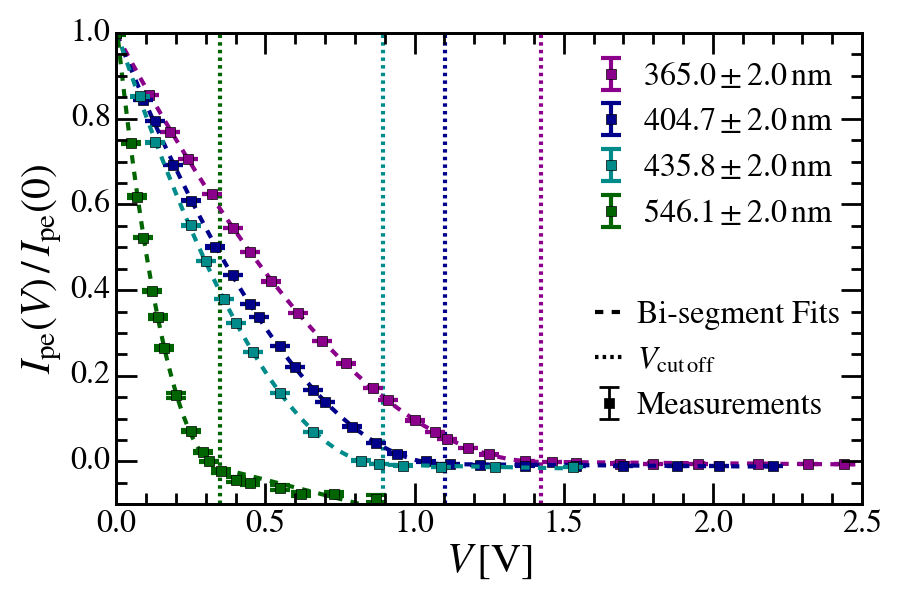
\includegraphics[width=0.49 \textwidth]{Figures/measurements.png}
    \caption{The photoelectric currents $I_{\rm{pe}}$ as functions of the retarded voltage $V$ for different wavelengths. For clarity of visualization, the currents are normalized by the initial photoelectric current at $V=0\V$. The dashed lines represent the bi-segment fits to the data, with the cutoff voltages $V_{\rm{cut\,off}}$ marked by the vertical dotted lines. For $\lambda = 546.1\nm$, the current curve appears to dip further below $I_{pe} = 0\pA$ when compared to in other wavelengths. This is mainly due to the limited initial current at the wavelength. Otherwise, the photoelectric currents behave consistently with expectations, with the cutoff voltage decreasing as wavelength increases. }
    \label{fig:measurements}
\end{figure}

\begin{table}
    \centering
    \addtolength{\tabcolsep}{3pt}
    \def\arraystretch{1.5}
    \begin{tabular}{c c c}
        \hline
        $\lambda$ & $V_{\rm{cut\,off}}$ & $\sim I_{\rm{pe}} (V_{\rm{cut\,off}})$ \\ [0ex]
        $[\rm{nm}]$ & $[\rm{V}]$ & $[\rm{pA}]$ \\ [1ex]
        \hline\hline

        $365.0 \pm 2.0$ & $1.425 \pm 0.010$ & $- 1.2$ \\
        $404.7 \pm 2.0$ & $1.104 \pm 0.014$ & $- 2.2$ \\
        $435.8 \pm 2.0$ & $0.892 \pm 0.015$ & $- 4.2$ \\
        $546.1 \pm 2.0$ & $0.366 \pm 0.059$ & $- 0.8$ \\
        \hline
        
    \end{tabular}
    \caption{The cut off voltages $V_{\rm{cut\,off}}$ at different wavelengths, along with the approximated photoelectric currents $I_{\rm{pe}}$ at the cut off voltages. The uncertainties are estimated from the standard deviations of the Monte Carlo sample fits, while the systematic errors $\sigma_{V_{\rm{cut\,off}}}^{\rm{sys}} \sim 0.04\V$ are taken as the difference in values between different approaches. The photoelectric currents are estimated from the bi-segment fits to the data and should be treated only as rough approximations.}
    \label{tab:cut_off_voltages}    
\end{table}

The photoelectric currents' dependencies on the retarded voltages are displayed in Fig.~\ref{fig:measurements}. The currents behave in accordance with the expectations discussed in Subsection~\ref{sec:data_collection}, i.e. exhibiting a gradual decrease as the voltage increases and finally reaching a plateau region beyond the cutoff voltage $V_{\rm{cut\,off}}$ in the reverse current regime. Different approaches are employed in order to obtain the values of the cutt of voltages. These include finding the intersection between the linear fits of the plateau and photoelectric (defined as the region of significant photoelectric currents) regimes, calculating the voltage at which the current reaches zero via functional fitting, or identifying the point where the current significantly deviates from the plateau. Here, we observe non-trivial curves in the photoelectric regime, as well as a non-zero slope in the plateau regime. Additionally, we notice that the photoelectric currents typically dip further below $I_{\rm{pe}} = 0\pA$ before trasitioning into a linear dependency of the retarded voltage. As a result, we decide to use bi-segment fits to characterize the photoelectric currents, with the cutoff voltages $V_{\rm{cut\,off}}$ function as the boundaries between regimes.

Such bi-segment fits comprise of a polynomial of order $n$ in the photoelectric regime and a linear function in the plateau regime. The two segments are connected in a maner such that $I_{\rm{pe}}$ and ${\rm{d}}I_{\rm{pe}} / {\rm{d}}V$ are continuous. This means that the bi-segment fit is effectively controlled by the polynomial coefficients $\boldsymbol{p}_n$. In order to identify the most expressive polynomial order $n$ while avoiding overfitting, we perform the Chow test~\citep{Chow1960} for polynomial fitting using the data with positive currents. In this context, the Chow test compares the RSS of different order polynomial and decides if the improvement in the fit is significant enough to justify the increase in the number of parameters via the f-statistic
\begin{equation}
    \label{eqn:chow_f_stat}
    F_{n,n^{\prime}} = \frac{(\chi^2_{n^{\prime}} - \chi^2_{n}) / (n - n^{\prime})}{\chi^2_n / (N - n)},
\end{equation}
for $n > n^{\prime}$. If $F_{n,n^{\prime}}$ is larger than the critical value $F_{\alpha=0.05}$, then the polynomial of order $n$ is considered to be a better fit. We perform the test and find that the best polynomial order is $n=3$ for all wavelengths. The bi-segment fits using the maximum likelihood approach are then implemented. The results are displayed in Fig.~\ref{fig:measurements}. Quanlitatively, the fits are well behaved, with the cutoff voltages $V_{\rm{cut\,off}}$ approximately manifesting at near the points where currents turn to zero. Qualitatively, it is hard to make sense of the RSS $\chi^2$ values, as the typical signal-noise ratio (SNR) of the photoelectric currents are relatively high ${\rm{SNR}} \sim 100$. This results in abnormally large values of $\chi^2$ and the fitting uncertainties approaching zero, which is not ideal. To obtainthe uncertainties in the cut off voltage $V_{\rm{cut\,off}}$, as well as to taken into account the uncetainties/limited resolution in the voltage measurements, we perform Monte Carlo sample fits, where from the initial data, we generate 10000 samples of retarded volatge $V$ according to the uniform distributions centering around the measured values with the width of $0.01\V$. The bi-segment fits are then performed on these samples. The central values and standard deviations of the cutoff voltages are calculated. The results are summarized in Table~\ref{tab:cut_off_voltages}, with the more detailed distributions of $V_{\rm{cut\,off}}$ present in Appendix~\ref{app:MC_fitting}. Here, we estimate the systematic errors as the typical deviation of the cut off voltages from the points at which the photoelectric currents reache zero, which are of the order of $\sigma_{V_{\rm{cut\,off}}}^{\rm{sys}} \sim 0.04\V$.

\subsection{Plank Constant and Work Function}
\label{sec:plank_constant}

\begin{figure}
    \centering
    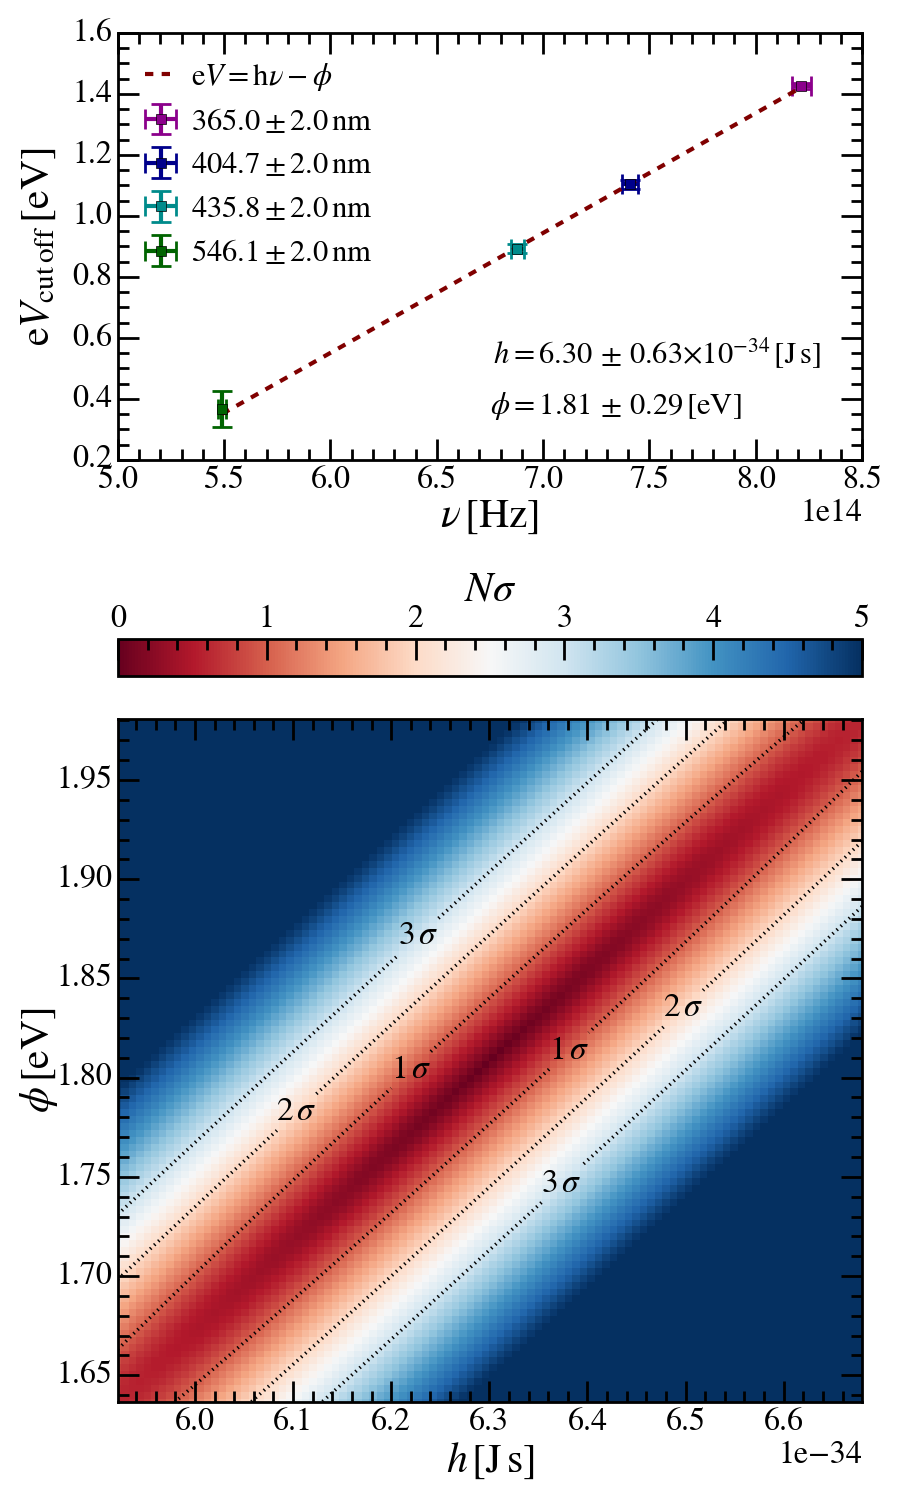
\includegraphics[width=0.49 \textwidth]{Figures/plank_and_work_function_fit.png}
    \caption{The fitting results of the Plank constant $h$ and the work function $\phi$ using the cut off voltages $V_{\rm{cut\,off}}$ measured in Table~\ref{tab:cut_off_voltages}. The dashed lines represent the best fit using the NLL following Equation~\ref{eqn:plank_NLL}, which results in the value of $h$ and $\phi$ as shown. The large uncertainties here are due to the degeneracy and correlation between $h$ and $\phi$, as displayed in the Gaussian-equivalent deviation (Equation~\ref{eqn:plank_uncertainty}) of the lower panel. This arise from the limited range of wavelength, as well as the large uncertainty of the cut off voltage at $\lambda = 546.1\nm$. The systematic errors of $h$ and $\phi$ are propagrated from $\sigma_{V_{\rm{cut\,off}}}^{\rm{sys}}$ and are estimated to be $\sim 5\%$.}
    \label{fig:h_and_phi}
\end{figure}

To obtain the Plank constant $h$ and the work function $\phi$, we utilize the photoelectric effect equation (Equation~\ref{eqn:work_function}) and the cutoff voltages $V_{\rm{cut\,off}}$ measured in Table~\ref{tab:cut_off_voltages}. Our prior then follows as
\begin{equation}
    \label{eqn:plank_prior}
    e \hat{V}_{\rm{cut\,off}} (\nu) = {\rm{h}} \nu - \phi,
\end{equation}
with $e$ as the electron charge. As there exist uncertainties in both the cut off voltage $V_{\rm{cut\,off}}$ and the wavelengths $\lambda$, we fit the data by minimizing the negative log likelihood (NLL)
\begin{equation}
    \label{eqn:plank_NLL}
    - 2 \log{\mathcal{L} (h,\phi)} = \sum_i \frac{\left(V_{\rm{cut\,off},i} - \hat{V}_{\rm{cut\,off}} (\nu_i)\right)^2}{\sigma_{V_{\rm{cut\,off},i}}^2 + \left(\frac{\partial \hat{V}_{\rm{cut\,off}} (\nu_i)}{\partial \nu} \right)^2 \sigma_{\nu_i}^2}.
\end{equation}
Approximating the likelihood to be Gaussian in the vicinity of the optimized value, we can calculate the fitting uncertainties using the inversion of the covariance matrix
\begin{equation}
    \label{eqn:plank_cov}
    \left(C\right)^{-1}_{\theta,\theta^{\prime}} \approx - \frac{\partial^2 \log{\mathcal{L}}}{\partial \theta \, \partial \theta^{\prime}},
\end{equation}
with $\theta$ and $\theta^{\prime}$ being either $h$ or $phi$. The Gaussian-equivalent uncertainty $N \sigma$ is then calculated as
\begin{equation}
    \label{eqn:plank_uncertainty}
    N^2 = \sum_{\theta,\theta^{\prime}} \left(\theta - \theta_0\right) \left(C\right)^{-1}_{\theta,\theta^{\prime}} \left(\theta^{\prime} - \theta^{\prime}_0\right).
\end{equation}
$\theta_0$ and $\theta^{\prime}_0$ are the optimized values of $\theta$ and $\theta^{\prime}$, respectively. The fitting results are displayed in Fig.~\ref{fig:h_and_phi}. We obtain the values of $h = 6.30 \pm 0.63 \times 10^{-34}\Js$ and $\phi = 1.81 \pm 0.29\ev$. These quoted uncertainties are calculated from the diagonal elements of the covariance matrix $C$, which in this case is deceptive, as there appears to be a strong degeneration and correlation between $h$ and $\phi$. These phenomena arise from the limited range of wavelength of our experiment, as well as the large uncertainty in the cutoff voltage of the longest wavelength $\lambda = 546.1\nm$. The systematic errors of $h$ and $\phi$ are mainly carried over from the errors of the cut off voltage measurement and are estimated to be $\sim 5\%$, resulting in $\sigma_h^{\rm{sys}} = 0.32\Js$ and $\sigma_\phi^{\rm{sys}} = 0.18\ev$.


\section{Discussion and Conclusion}
\label{sec:conclusion}

In this paper, we present a measurement of the Plank constant $h$ and the work function of the material $\phi$ from the cut off volatges $V_{\rm{cut\,off}}$ at different wavelengths. We obstain the value of $h = 6.30 \pm 0.63^{\rm{stat}} \pm 0.32^{\rm{sys}} \times 10^{-34}\Js$ and $\phi = 1.81 \pm 0.29^{\rm{stat}} \pm 0.18^{\rm{sys}}\ev$.

The cut off voltages are measured from the photoelectric currents $I_{\rm{pe}}$ as functions of the retarded voltages $V$ for the wavelengths of $\lambda = 365.0, \, 404.7, \, 435.8,$ and $546.1\nm$. The values of $V_{\rm{cut\,off}}$ are determined by bi-segment fits to the photoelectric currents, with the results summarized in Table~\ref{tab:cut_off_voltages}. The systematic errors of $V_{\rm{cut\,off}}$ are estimated to be $\sim 0.04\V$. This systematic error arises from the difference between the obtained values of $V_{\rm{cut\,off}}$ from the different approaches. The statistical errors, on the other hand, are calculated from the Monte Carlo sample fits and are of the order of $\sim 0.01\V$. The cutoff voltages decrease as the wavelength increases, which is consistent with the expectations of the photoelectric effect.

For the fitting of the Plank constant $h$ and the work function $\phi$, we observe that the statistical uncertainties are relatively large, as the consequence of $h$ and $\phi$ being correlated, which, in turn, arise from the limited range of wavelengths and the large uncertainty in the cut off voltage at $\lambda = 546.1\nm$. The systematic errors of $h$ and $\phi$ are mainly due to the uncertainties in the cutoff voltage measurements and are estimated to be $\sim 5\%$. The value of $h$ is relatively consistent with the literature value of $h = 6.63 \times 10^{-34}\Js$.

In our future work, we intend to include the use of a more precise apparatus to reduce the uncertainties in the measurements. Additionally, we aim to expand the range of wavelengths in order to reduce the correlation between the fitted values of $h$ and $\phi$. We also plan to investigate the effects of the background currents on the measurements, as well as to explore the possibility of using a more sophisticated fitting approach to reduce uncertainties.

\begin{acknowledgments}

The author thanks his lab partner J. Park for collaboration in the experiment, as well as Y. Hu for support in the formatting and structuring of the manuscript. The author also thanks the JLab teaching staffs for their guidance and support, as well as the MIT Physics Department for providing the experimental apparatus.

\end{acknowledgments}

%%%%%%%%%%%%%%%%%%%%%%%%%%%%%%%%%%%%%%%%%%%%%%%%%%%%%%%%%%%%%%%%%%

\bibliography{main}

%%%%%%%%%%%%%%%%%%%%%%%%%%%%%%%%%%%%%%%%%%%%%%%%%%%%%%%%%%%%%%%%%%

\appendix

\section{Monte Carlo Sample Fits}
\label{app:MC_fitting}

\begin{figure}
    \centering
    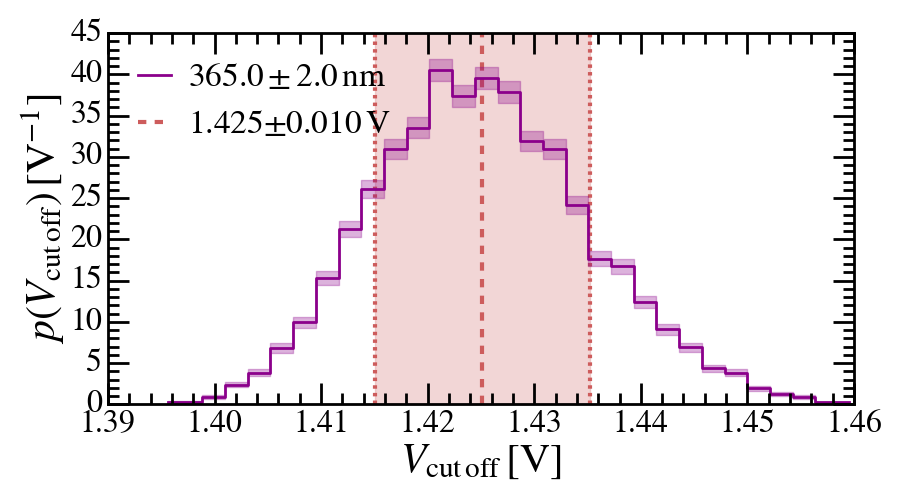
\includegraphics[width=0.49 \textwidth]{Figures/V_cutoff_365nm.png}
    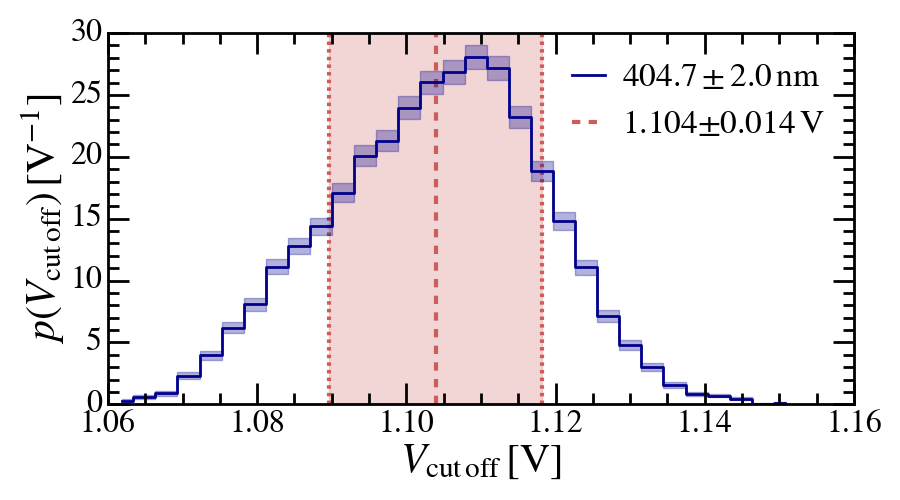
\includegraphics[width=0.49 \textwidth]{Figures/V_cutoff_405nm.png}
    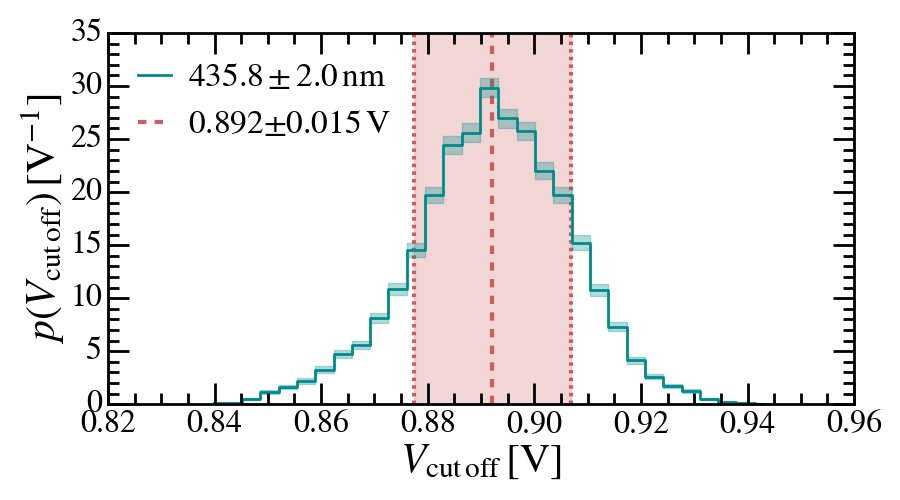
\includegraphics[width=0.49 \textwidth]{Figures/V_cutoff_436nm.png}
    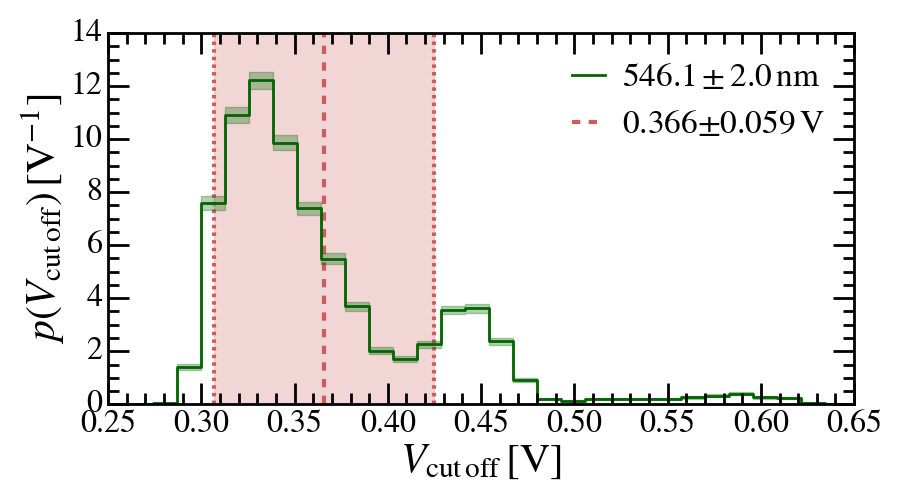
\includegraphics[width=0.49 \textwidth]{Figures/V_cutoff_546nm.png}
    \caption{The results of 10000 Monte Carlo sample fits for the cut off voltage at different wavelengths, following the procedure described in Section~\ref{sec:result}. The histograms show the distribution of the cutoff voltage $V_{\rm{cut\,off}}$, while the dashed red line and shaded regions represent the central fitted values and their standard deviations. For the three shorter wavelengths, the fits are generally well behaved, with a unimodal Gaussian-like distribution. On the other hand, the longest wavelength of $546.1\nm$ shows a bimodal distribution, which may be the result of the limited measurements. The central value and standard deviation of the cutoff voltage for this particular wavelength reflect the bimodal distribution.}
    \label{fig:MC_fitting}
\end{figure}

\end{document}